\chapter{Testrig}
\section{Introduction}

\section{Requiremens}

\subsection{Motor requirements}
Modeled negative forces acting on vehicle (gravity, air resistance, friction) with average speed of 6.96 m/s: 

\begin{figure}[H]
    \centering
    \label{fig:testrig_negative_forces}
    \includegraphics[width=0.5\textwidth]{./testrig/negative_forces.eps}
    \caption{Negative forces acting upon Elba in one lap.}
\end{figure}

Torque required on wheel of Elba:
$$T_w = F_n\*r_w$$

Torque required for roller on test rig:
$$T_r = \frac{T_w\*r_r}{r_w}$$

Required torque for motor, $T_m$:
$$T_m = T_t + J_r\*\ddot{\phi} + d\*\dot{\phi}_m + k\*\phi_m$$

Power required for motor:
$$P_m = T_m\*\dot{\phi}_m$$

The inertia $J_r$ for the rollers on the testrig was calculated to be $0.0039$ $kgm^2$

This results in $P_m = 1000$ W

\begin{figure}[H]
    \centering
    \label{fig:testrig_power_required_motor}
    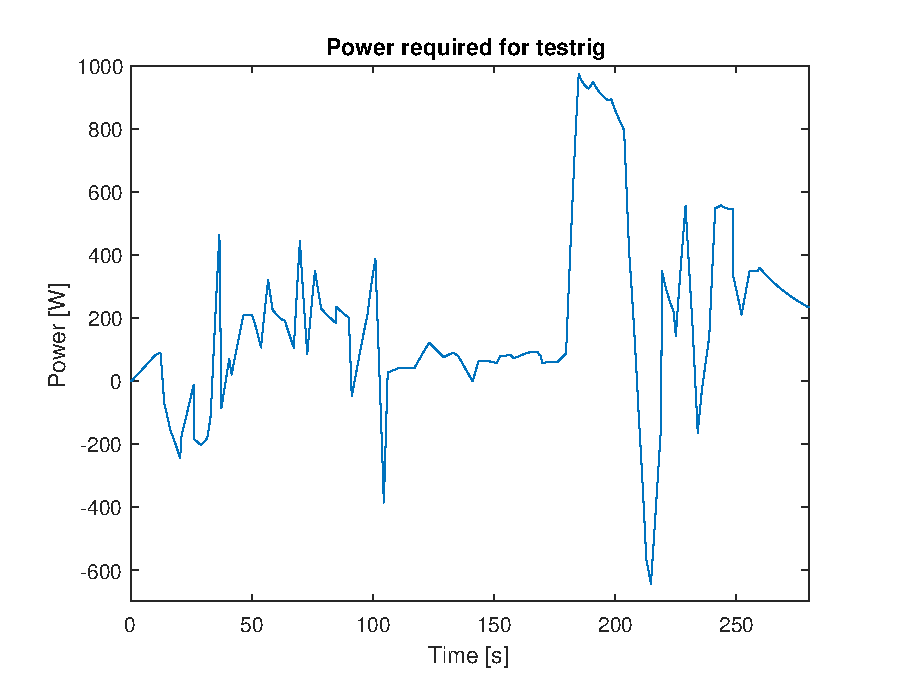
\includegraphics[width=0.5\textwidth]{./testrig/power_required_testrig.eps}
    \caption{Power required for the motor on the testrig.}
\end{figure}
